\subsection{Construction of Fiber Bundles}

\begin{definition}[Fiber Bundle]
    \label{fiber_bundles:def:fiber_bundle}
    Let $G$ be a topological group acting effectively on a space $F$. A fiber bundle $E$ over $B$ with fiber $F$ and structure group $G$ consists of a surjective continuous map $p \colon E \to B$ and a collection of maps 
    \[
    (\phi_\alpha \colon U_\alpha \times F \to p^{-1}(U_\alpha))_\alpha,
    \]
    called a trivialising atlas\footnote{Wikipedia calls this a \textit{G-Atlas}}, for open sets $U_\alpha \subseteq B$, such that 
    \begin{enumerate}[(i)]
        \item The maps $\phi_\alpha$ are homeomorphisms and the following diagrams commute:
        \begin{center}
            \commtriangle{$U_\alpha\times F$}{$p^{-1}(U_\alpha)$}{$U_\alpha$}{$\phi_\alpha$}{$\pi$}{$p$}
        \end{center}
        where $\pi$ is the usual projection onto the first factor.
        \item For any two maps $\phi_\alpha, \phi_\beta$ there exists a continuous map
        \[
        \tau_{\alpha,\beta} \colon U_\alpha \cap U_\beta \to G,
        \]
        such that
        \[
        \phi_\alpha^{-1} \circ \phi_\beta \colon (U_\alpha \cap U_\beta) \times F \to (U_\alpha \cap U_\beta) \times F
        \]
        is given by $(b,f) \mapsto (b,\tau_{\alpha,\beta} \cdot f)$.
        \item $(U_\alpha)_\alpha$ is an open cover of $B$.
        \item The collection $(\phi_\alpha)$ is maximal with respect to the first 3 conditions.
    \end{enumerate}
    The maps $\phi_\alpha$ are called local trivialisations,  the sets $U_\alpha$ are called trivialising neighbourhoods and the map $\tau_{\alpha,\beta}$ is called the transition function for $\phi_\alpha,\phi_\beta$. We write $(U_\alpha,\phi_\alpha)$ as a shorthand for the local trivialisation $\phi_\alpha \colon U_\alpha \times F \to p^{-1}(U_\alpha)$. Furthermore, we call $E$ the total space, $B$ the base space and $F$ the fiber. We denote the fiber bundle by
    \[
    F \hookrightarrow E \oset[0.5pt]{\scalebox{0.8}{$p$}}{\longrightarrow} B
    \]
    or sometimes just by $E \xrightarrow{p} B$.  
\end{definition}

Fiber bundles with structure group also come with an appropriate notion of morphism:

\begin{definition}
    \label{fiber_bundles:def:bundle_morphism}
    Let $F \hookrightarrow E \oset[0.5pt]{\scalebox{0.8}{$p$}}{\longrightarrow} B$ and $F \hookrightarrow E^\prime \oset[0.5pt]{\scalebox{0.8}{$p$}}{\longrightarrow} B^\prime$ be fiber bundles with structure group $G$. A $G$-morphism is a pair $(H,h)$ of continuous maps $H \colon E \to E^\prime$ and $h \colon B \to B^\prime$, such that 
        \[\begin{tikzcd}
        E & {E^\prime} \\
        B & {B^\prime}
        \arrow["H", from=1-1, to=1-2]
        \arrow[from=1-1, to=2-1]
        \arrow[from=1-2, to=2-2]
        \arrow["h", from=2-1, to=2-2]
        \end{tikzcd}\]
        commutes and in local trivialisations $H$ is given by the action of elements in $G$. That is for any local trivialisations $(U_\alpha,\phi_\alpha)$ of $E$ and $(V_\beta,\psi_\beta)$ of $E^\prime$ with $h(U_\alpha) \subseteq V_\beta$ there exists a continuous map 
        \[
        g_{\alpha\beta} \colon U_\alpha \to G,
        \] 
        such that the composition $\psi_\beta^{-1} \circ H \circ \phi_\alpha \colon U_\alpha \times F \to V_\beta \times F$ is given by 
        \[
        (x,f) \mapsto (h(x),g_{\alpha\beta}(x) \cdot f).
        \]
        We usually denote such a morphism only by $H \colon E \to E^\prime$. Note that $h$ is completely determined by $f$, justifying this notation. If $B = B^\prime$ we generally implicitly require $h$ to be the identity. 
\end{definition}

Note that with the above definition any $G$-morphism is a fiber wise homeomorphism. Sometimes we may want to relax this condition by dropping the requirement that locally $H$ is given by the action of group elements and call the resulting morphism simply a morphism of fiber bundles. For categoy theoretical aspects it is however nicer to work with $G$-morphisms. Thus we define the category $\mathsf{Fib}_{F,G}$ to be the category whose objects are given by fiber bundles with fiber $F$ and structure group $G$ and whose morphisms are given by $G$-morphisms.

\begin{remark}
    In Definition \ref{fiber_bundles:def:fiber_bundle} we require surjectivity of $p$ to exclude the case $F = \emptyset$. The requirement, that $G$ acts effectively guarantees for the transition maps to be unique. However, this is not a strong requirement to impose, since if $G$ does not act effectively, i.e.
    \[
    \Phi \colon G \to \mathrm{Aut}(F)
    \]
    is not injective we get an effective group action by taking a quotient of $G$:
    \[
    G/\mathrm{ker}\Phi \to \mathrm{Aut}(F).
    \]
    It follows from the universal property of the quotient topology, that $G/\mathrm{ker}\Phi$ still acts continuously on $F$, i.e. the induced map $G/\mathrm{ker}\Phi \times F \to F$ is still continuous (if $F$ is locally compact we can define the exponential topology on Aut$(F)$ and the statement is equivalent to $G/\mathrm{ker}\Phi \to \mathrm{Aut}(F)$ being continuous).
\end{remark}

\begin{remark}
    The maximality condition for the trivialising atlas is well-defined: Given any trivialising atlas $\mathcal{F} = (\phi_\alpha)_\alpha$ satisfying conditions (i) - (iii) of Definition \ref{fiber_bundles:def:fiber_bundle} we can define
    \begin{align*}
        \hat{\mathcal{F}} := \{& \phi \colon U \times F \to p^{-1}(U) \mid U \subseteq B \text{ open }, \phi \text{ homeomorphism},  \text{ for any } \phi_\alpha \in \mathcal{F} \\ &\text{exists a map } \tau_{\alpha,\phi} \colon U \cap U_\alpha \to G, \text{ with } (\phi_\alpha^{-1} \circ \phi)(b,f) = (b,\tau_{\alpha,\phi}(b) \cdot f) \}.
    \end{align*}
    This is the maximal trivialising atlas induced by $\mathcal{F}$ satisfying (i) - (iii). Note however, that there is no unique trivialising atlas, since beginning with a different $\mathcal{F}$ may yield a different $\hat{\mathcal{F}}$ (as is the case for smooth atlases of smooth manifolds).
    \begin{proof}[Proof of above remark]
        Given $\phi \colon U \times F \to p^{-1}(U), \phi^\prime \colon U^\prime \times F \to p^{-1}(U^\prime) \in \hat{\mathcal{F}}$, we claim that there exists $\tau \colon U \cap U^\prime \to G$, such that
        \[
        (\phi^{-1} \circ \phi^\prime)(b,f) = (b,\tau(b) \cdot f).
        \]
        For $b_0 \in B$ choose $(\phi_\alpha \colon U_\alpha \times F \to p^{-1}(U_\alpha)) \in \mathcal{F}$ with $b_0 \in U_\alpha$. Then there exists
        \[
        \tau_{\alpha,\phi} \colon U \cap U_\alpha \to G, \; \tau_{\alpha,\phi^\prime} \colon U^\prime \cap U_\alpha \to G
        \]
        with
        \[
        (\phi^{-1}_\alpha \circ \phi)(b,f) = (b,\tau_{\alpha,\phi}(b) \cdot f), \; 
        (\phi^{-1}_\alpha \circ \phi^\prime)(b,f) = (b,\tau_{\alpha,\phi^\prime}(b) \cdot f).
        \]
        Then
        \[
        (\phi^{-1} \circ \phi_\alpha) \circ (\phi_\alpha^{-1} \circ \phi^\prime) \colon (U_\alpha \cap U \cap U^\prime) \times F \to (U_\alpha \cap U \cap U^\prime) \times F 
        \]
        is given by
        \[
        (b,f) \mapsto (b, \tau_{\alpha,\phi}(b)^{-1}\tau_{\alpha,\phi^\prime}(b) \cdot f).
        \]
        We conclude that around $\{b_0\} \times F$ we have
        \[
        (\phi^{-1} \circ \phi^\prime)(b,f) = (b,\tau(b) \cdot f)
        \]
        for $\tau(b) := \tau_{\alpha,\phi}(b)^{-1}\tau_{\alpha,\phi^\prime}(b)$. Since group inversion and multiplication are continuous, $\tau$ is continuous. As $b_0$ was chosen arbitrary, such a map $\tau$ can be defined on all of $U \cap U^\prime$. Furthermore, the group action of $G$ is effective, hence $\tau$ is unique and the above argument shows that it is continuous. 
    \end{proof}
\end{remark}

    For the transition functions we have the following Lemma, where again the effectiveness of the group action is crucial.

    \begin{lemma}
        \label{lem:transition_functions}
        Let $F \hookrightarrow E \oset[0.5pt]{\scalebox{0.8}{$p$}}{\longrightarrow} B$ be a fiber bundle with structure group $G$. Then (using the notation in Definition \ref{fiber_bundles:def:fiber_bundle}):
        \begin{enumerate}[(i)]
            \item $\tau_{\alpha,\alpha}(b) = e$
            \item $\tau_{\alpha,\beta}^{-1}(b) = \tau_{\beta,\alpha}(b)$
            \item $\tau_{\gamma,\alpha}(b)\tau_{\alpha,\beta}(b) = \tau_{\gamma,\beta}(b)$
        \end{enumerate}
    \end{lemma}
    \begin{proof}
        Let us first proof (iii), then (i) and (ii) follow directly from the group axioms. We compute:
        \begin{align*}
            (b,\tau_{\gamma,\beta}(b) \cdot f) & = (\phi_\gamma^{-1} \circ \phi_\beta)(b,f) \\ & = (\phi_\gamma^{-1} \circ \phi_\alpha \circ \phi_\alpha^{-1} \circ \phi_\beta)(b,f) = (b,\tau_{\gamma,\alpha}(b)\tau_{\alpha,\beta}(b) \cdot f).
        \end{align*}
        Since the transition functions are uniquely determined, the statement follows. 
    \end{proof}

     Interestingly, the transition functions already uniquely determine the fiber bundle, in a sense made precise by the following theorem.

     \begin{theorem}[Fiber bundle construction A]
        \label{fiber_bundles:thm:fiber_bundle_construction1}
        Let $B,F$ be (non-empty) topological spaces and $G$ a topological group acting effectively on $F$. Suppose we are given the following data:
        \begin{enumerate}[(i)]
            \item An open cover $\mathcal{U} := (U_\alpha)_\alpha$ of B (where $\alpha$ ranges over some index set $A$)
            \item A collection $(\tau_{\alpha,\beta})$ of continuous maps
            \[
            \tau_{\alpha,\beta} \colon U_\alpha \cap U_\beta \to G
            \]
            for each pair $U_\alpha,U_\beta \in \mathcal{U}$
            \item $\tau_{\gamma,\alpha}(b)\tau_{\alpha,\beta}(b) = \tau_{\gamma,\beta}(b)$ for all $b \in U_\alpha \cap U_\beta \cap U_\gamma$
        \end{enumerate}
        Then there exists a unique (up to isomorphism) fiber bundle $F \hookrightarrow E \oset[0.7pt]{\scalebox{0.8}{$p$}}{\longrightarrow} B$ with structure group $G$, such that the maximal trivialising atlas is induced by a trivialising atlas of the form
        \[
        (\phi_\alpha \colon U_\alpha \times F \to p^{-1}(U_\alpha))_\alpha,
        \]
        such that $(\phi_\alpha^{-1} \circ \phi_\beta)(b,f) = (b,\tau_{\alpha,\beta}(b) \cdot f)$.
     \end{theorem}
     \needspace{8\baselineskip}
     \begin{proof}
        Consider the space
        \[
        E := \left( \coprod_{\alpha \in A} U_\alpha \times F \right)_{\raisebox{5pt}{\scalebox{1.5}{$/$}}\raisebox{5pt}{\scalebox{1.05}{$\sim$}}}
        \]
        where the equivalence relation $\sim$ is defined by
        \[
        (b,f,\beta) \sim (b,\tau_{\alpha,\beta}(b) \cdot f,\alpha)
        \]
        and let $p \colon E \to B, \: [(b,f,\alpha)] \mapsto b$. Furthermore, let $\pi \colon \raisebox{1.2pt}{$\scalebox{0.8}{$\coprod$}_\alpha$} \, U_\alpha \times F \to E$ be the projection map.

        \textbf{Step 1.} \textit{$\sim$ is an equivalence relation.}

        Transitivity follows directly from condition (iii). Reflexivity and symmetry then follow from the group axioms.

        \textbf{Step 2.} \textit{$p$ is well-defined, continuous and surjective.}

        Clearly $p$ is well-defined and surjective as $F \neq \emptyset$. Continuity then follows directly from the universal property of the quotient topology.

        \textbf{Step 3.} \textit{Defining the trivialising atlas}

        Consider
        \[
        \phi_\alpha \colon U_\alpha \times F \to p^{-1}(U_\alpha), \; (b,f) \mapsto [(b,f,\alpha)].
        \]
        Clearly $\phi_\alpha$ is well-defined ($[(b,f,\alpha)] \in p^{-1}(U_\alpha)$) and continuous (the projection map $\pi$ is continuous). The inverse is given by
        \[
        \phi_\alpha^{-1}([(b,f,\beta)]) = (b,\tau_{\alpha,\beta}(b) \cdot f).
        \]
        To show that $\phi_\alpha^{-1}$ is continuous, we show that $\phi_\alpha$ is an open map. To this end, let $U \times V \subseteq U_\alpha \times F$ be open and consider
        \[
        \theta_{\alpha,\beta} \colon (U_\alpha \cap U_\beta) \times F \to (U_\alpha \cap U_\beta) \times F, \; (b,f) \mapsto (b, \tau_{\alpha,\beta}(b) \cdot f). 
        \]
        Clearly $\theta_{\alpha,\beta}$ is continuous (in fact it is a homeomorphism), hence
        \[
        V_\beta := \theta_{\alpha,\beta}^{-1}((U \cap U_\beta) \times V) \subseteq (U_\alpha \cap U_\beta) \times F
        \]
        is open and thus
        \[
        \pi^{-1}(\phi_\alpha(U \times V)) = \coprod_{\beta \in A} V_\beta \subseteq \coprod_{\beta \in A} U_\beta \times F
        \]
        is open. Thus $\phi_\alpha(U\times V)$ is open in $E$ and since $p^{-1}(U_\alpha)$ is also open, we conclude that $\phi_\alpha$ is an open map. Furthermore, the diagram
        \begin{center}
            \commtriangle{$U_\alpha\times F$}{$p^{-1}(U_\alpha)$}{$U_\alpha$}{$\phi_\alpha$}{}{$p$}
        \end{center}
        commutes, such that $\phi_\alpha$ is a local trivialisation. Moreover,
        \[
        (\phi_\alpha^{-1} \circ \phi_\beta)(b,f) = (b,\tau_{\alpha,\beta}(b) \cdot f).
        \]
        So the collection of maps $(\phi_\alpha)_\alpha$ is a trivialising atlas with the desired transition functions, making $F \hookrightarrow E \oset[0.6pt]{\scalebox{0.8}{$p$}}{\longrightarrow} B$ into a fiber bundle with structure group $G$.

        \textbf{Step 4.} \textit{Uniqueness}

        Given two fiber bundles
        \begin{align*}
            \delta & := (F \hookrightarrow E \oset[0.6pt]{\scalebox{0.8}{$p$}}{\longrightarrow} B) \\
            \epsilon & := (F \hookrightarrow \tilde{E} \oset[2pt]{\scalebox{0.8}{$\tilde{p}$}}{\longrightarrow} B)
        \end{align*}
        with structure group $G$ and trivialising atlases
        \begin{align*}
            (\phi_\alpha \colon U_\alpha \times F \to p^{-1}(U_\alpha))_{\alpha \in A} \\
            (\tilde{\phi}_\alpha \colon U_\alpha \times F \to \tilde{p}^{-1}(U_\alpha))_{\alpha \in A}
        \end{align*}
        respectively, such that
        \[
        (\phi_\alpha^{-1} \circ \phi_\beta) (b,f) = (b,\tau_{\alpha,\beta}(b) \cdot f) = (\tilde{\phi}_\alpha^{-1} \circ \tilde{\phi}_\beta) (b,f).
        \]
        We can then construct an isomorphism $\Gamma \colon \delta \to \epsilon$ as follows: for $x \in E$ choose $U_\alpha \in \mathcal{U}$ with $p(x) \in U_\alpha$. Then define
        \[
        \Gamma(x) := (\tilde{\phi}_\alpha \circ \phi_\alpha^{-1})(x).
        \]
        Well-definedness of $\Gamma$ follows from the commutativity of the following diagram:
        \begin{center}
            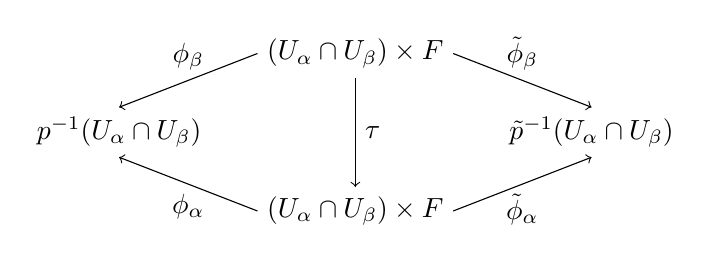
\begin{tikzpicture}
                \draw node (left) at (-3,0) {$p^{-1}(U_\alpha \cap U_\beta)$};
                \draw node (up) at (0,1) {$(U_\alpha \cap U_\beta) \times F$};
                \draw node (down) at (0,-1) {$(U_\alpha \cap U_\beta) \times F$};
                \draw node (right) at (3,0) {$\tilde{p}^{-1}(U_\alpha \cap U_\beta)$};

                \draw[->] (up.west) to node[above]{$\phi_\beta$} (left.north);
                \draw[->] (down.west) to node[below] {$\phi_\alpha$} (left.south);
                \draw[->] (up.east) to node[above] {$\tilde{\phi}_\beta$} (right.north);
                \draw[->] (down.east) to node[below] {$\tilde{\phi}_\alpha$} (right.south); 
                \draw[->] (up.south) to node[right] {$\tau$} (down.north);
            \end{tikzpicture}
        \end{center}
        where $\tau(b,f) := (b, \tau_{\alpha,\beta}(b) \cdot f)$. Locally $\Gamma$ is given by a continuous map, so it is continuous. Analogously we define the inverse map. Furthermore,
        \begin{center}
            \commtriangle{$E$}{$\tilde{E}$}{$B$}{$\Gamma$}{$p$}{$\tilde{p}$}
        \end{center}
        commutes, so $\Gamma$ is a bundle isomorphism. This completes the proof.
     \end{proof}

    \needspace{5em}
     We may also formulate Theorem \ref{fiber_bundles:thm:fiber_bundle_construction1} slightly different, if we are given the fibers $F_x = p^{-1}(x)$ as sets. This is usually more practical, as the description of the bundle is more explicit:

     \begin{theorem}[Fiber bundle construction B]
        \label{thm:fiber_bundle_construction2}
        Let $B,F$ be (non-empty) topological spaces and $G$ a topological group acting effectively on $F$. Given sets $F_x$ for each $x \in B$ we define $$E := \coprod_{x \in B}F_x$$ and $p \colon E \to B$ by sending each element in $F_x$ to $x$. Suppose we are given the following data:
        \begin{enumerate}[(i)]
            \item An open cover $\mathcal{U} := (U_\alpha)_\alpha$ of B (where $\alpha$ ranges over some index set $A$)
            \item A collection of bijections $\phi_\alpha \colon U_\alpha \times F \to p^{-1}(U_\alpha)$, that restrict to bijections $\{x\} \times F \to F_x$
            \item  A collection $(\tau_{\alpha,\beta})$ of continuous maps
            \[
            \tau_{\alpha,\beta} \colon U_\alpha \cap U_\beta \to G
            \]
            for each pair $U_\alpha,U_\beta \in \mathcal{U}$, such that $(\phi_\alpha^{-1} \circ \phi_\beta)(b,f) = (b,\tau_{\alpha,\beta}(b) \cdot f)$
        \end{enumerate}
        Then $E$ has a unique topology making $F \hookrightarrow E \oset[0.6pt]{\scalebox{0.8}{$p$}}{\longrightarrow} B$ into a fiber bundle with structure group $G$, where the maps $\phi_\alpha$ are local trivialisations.
     \end{theorem}
     \begin{proof}
        Define the topology on $E$ as the final topology with respect to the maps $\phi_\alpha$, i.e.
        \[
        V \subseteq E \text{ is open } \Leftrightarrow \phi_\alpha^{-1}(V) \subseteq U_\alpha \times F \text{ is open for each } \alpha
        \]
        We show that the maps $\phi_\alpha$ are open with this topology. To this end, let $W \subseteq U_\alpha \times F$ be open. Then
        \[
        \phi_\beta^{-1}(\phi_\alpha(W)) = (\phi_\beta^{-1} \circ \phi_\alpha)(W \cap ((U_\alpha \cap U_\beta) \times F)) \subseteq U_\beta \times F
        \]
        is open, since $\phi_\beta \circ \phi_\alpha$ is a homeomorphism by condition (iii). Thus $\phi_\alpha$ is a homeomorphism. In particular, for any open set $U \subseteq U_\alpha$, we get that
        \[
        p^{-1}(U) = \phi_\alpha(U \times F)
        \]
        is open, since by (ii) the following diagram commutes:
        \begin{center}
            \commtriangle{$U_\alpha \times F$}{$p^{-1}(U_\alpha)$}{$U_\alpha$}{$\phi_\alpha$}{}{$p$}
        \end{center}
        So $p$ is also continuous. Moreover, as $F \neq \emptyset$, we get that $p$ is surjective. It remains to show uniqueness. So let $E$ be equipped with any topology, such that $p$ is continuous and $\phi_\alpha$ are homeomorphisms. Let $V \subseteq E$, such that 
        \[
        W_\alpha := \phi_\alpha^{-1}(V) \subseteq U_\alpha \times F
        \]
        is open for all $\alpha$. Then 
        \[
        V = \bigcup_\alpha W_\alpha,
        \]
        since the $U_\alpha$ cover $B$ (and hence $E = \bigcup_\alpha \mathrm{im}\phi_\alpha$). As the $\phi_\alpha$ are homeomorphisms and $p^{-1}(U_\alpha)$ is open, we conclude that $V$ is open. Furthermore, the topology can not be finer than the final topology defined above, such that the two must coincide.
     \end{proof}

     \begin{example}
        \label{fiber_bundles:example:frame_bundle}
        Suppose we are given a (toplogical) rank $n$ vector bundle $E \xrightarrow{\pi} B$. We can use Theorem \ref{thm:fiber_bundle_construction2} to define the \textbf{frame bundle} $\mathrm{GL}(E)$ of $E$ as follows. Let $\mathrm{GL}(E_x)$ denote the set of all ordered bases of the vector space $E_x := \pi^{-1}(x)$ and set 
        \[
        \mathrm{GL}(E) := \coprod_{x \in B} \mathrm{GL}(E_x).
        \]
        Now choose an open cover $(U_\alpha)$ of $B$ over which $E$ is trivial, i.e. there exist local frames $X_1^\alpha,\ldots,X_n^\alpha$ over $U_\alpha$. We define the local trivialisations for the bundle by 
        \begin{align*}
            \phi_\alpha \colon U_\alpha \times \mathrm{GL}(n) &\to p^{-1}(U_\alpha) \\
            (x,A) &\mapsto \left(\sum_{i=1}^n a_{i1}X_i^\alpha(x),\ldots,\sum_{i=1}^n a_{in}X_i^\alpha(x)\right),
        \end{align*}
        where $A = (a_{ij})$, i.e. $\phi_\alpha(x,A)$ is the basis of $E_x$, whose coordinates in the frame $(X_i^\alpha)$ are precisely the columns of the matrix $A$. Clearly $\phi_\alpha$ is a bijection. Moreover for $x \in U_\alpha \cap U_\beta$ we have 
        \[
        (\phi_\alpha^{-1} \circ \phi_\beta)(x,A) = (x,\tau_{\alpha,\beta}(x)A),
        \]
        where $\tau_{\alpha,\beta}(x) \in \mathrm{GL}(n)$ is the change of basis matrix from $(X_i^\beta(x))$ to $(X_i^\alpha(x))$, which depends continuously on $x$. So applying Theorem \ref{thm:fiber_bundle_construction2} we can see $\mathrm{GL}(E)$ as principal $\mathrm{GL}(n)$-bundle over $B$. Using Theorem \ref{thm:fiber_bundle_construction2_smooth} the same construction works in the smooth category. It is interesting to note that $E$ is trivial if and only if $\mathrm{GL}(E)$ admits a global section.
        
        If $E$ carries a fiber metric we may similiarly construct the \textbf{orthonormal frame bundle} $O(M)$ as a principal $\mathrm{O}(n)$-bundle and if $E$ is oriented we can construct the \textbf{oriented frame bundle} $\mathrm{GL^+}(M)$ as a principal $\mathrm{GL^+}(n)$-bundle. Of course we can also combine the two to get the \textbf{oriented orthonormal frame bundle} $\mathrm{SO}(M)$.
     \end{example}

     Theorem \ref{fiber_bundles:thm:fiber_bundle_construction1} describes a construction which can be applied to objects in $\mathsf{Fib}_{F,G}$. The following theorem describes an analgous construction for the morphisms, which is will be the key to the functoriality result of Theorem \ref{fiber_bundles:thm:change_of_fiber_functor} below.

     \begin{proposition}
        \label{fiber_bundles:prop:construction_of_morphisms}
        Let $E \to B$ and $E^\prime \to B^\prime$ be fiber bundles with fiber $F$ and structure group $G$. Suppose we are given the following data:
        \begin{enumerate}[(i)]
            \item A continuous map $f \colon B \to B^\prime$,
            \item Trivialisations $(U_\alpha,\phi_\alpha)_{\alpha}$ of $E$ and $(V_\beta,\psi_\beta)_{\beta}$ of $E^\prime$, such that the $U_\alpha$ cover $B$ and for each $\alpha$ there exists some $\beta$ with $f(U_\alpha) \subseteq V_\beta$,
            \item For each pair $\alpha,\beta$ with $f(U_\alpha) \subseteq V_\beta$ a continuous map $g_{\alpha\beta} \colon U_\alpha \to G$, which transforms as follows: for some other $\alpha^\prime,\beta^\prime$ with $f(U_{\alpha^\prime}) \subseteq V_{\beta^\prime}$ it holds that 
            \[
            g_{\alpha\beta}(x) = \tau^{-1}_{\beta^\prime\beta}(x) g_{\alpha^\prime\beta^\prime}(x) \tau_{\alpha^\prime\alpha}(x)
            \]
            for all $x \in U_\alpha \cap U_{\alpha^\prime}$, where $\tau_{\alpha^\prime\alpha}$ and $\tau_{\beta^\prime\beta}$ are the respective transition functions.
        \end{enumerate}
        Then there exists a unique $G$-morphism $E \to H$, which corresponds to the maps 
        \[
        U_\alpha \times F \to V_\beta \times F, \; \; (x,f) \mapsto (f(x), \, g_{\alpha\beta}(x) \cdot f)
        \]
        under the local trivialisations $\phi_\alpha$ and $\psi_\beta$ for all $\alpha, \beta$ with $f(U_\alpha) \subseteq V_\beta$.     \end{proposition}

        \begin{proof}
            By definition any $G$-morphism is locally determined by maps $g_{\alpha\beta} \colon U_\alpha \to G$ and these maps transform as in $(iii)$ by definition of the transition functions. So conversely we may define a $G$-morphism locally by these $g_{\alpha\beta}$ and since they transform correctly we get a globally defined object.
        \end{proof}

        \headline{Smooth Bundles}

        \noindent If we are in the smooth category, we can analogously define smooth fiber bundles by requiring the spaces $E ,B$ and $F$ to be smooth manifolds (where either $F$ or $B$ has no boundary), the group $G$ to be a Lie group and all maps to be smooth. In particular, the local trivialisation are diffeomorphisms. All of the above results also hold in the smooth category. 

    \begin{theorem}[Fiber bundle construction $\mathrm{A}^\prime$]
        The conclusions of Theorem \ref{fiber_bundles:thm:fiber_bundle_construction1} remain true in the smooth category. 
    \end{theorem}
    \begin{proof}
        The only difficulty is in defining the smooth structure on 
        \[
            E := \left( \coprod_{\alpha \in A} U_\alpha \times F \right)_{\raisebox{5pt}{\scalebox{1.5}{$/$}}\raisebox{5pt}{\scalebox{1.05}{$\sim$}}}
        \]
        This smooth structure is defined via the local trivialisations $(\phi_\alpha)$ as follows: Choose and open cover $(V_\alpha)$ of $B$, such that
        \begin{itemize}
            \item $V_\alpha \subseteq U_\alpha$
            \item there exist smooth charts $h_\alpha \colon W_\alpha \to V_\alpha$
        \end{itemize}
        Furthermore, choose a smooth atlas
        \[
        (k_i \colon W_i^F \to V_i^F)_i
        \]
        of $F$. Then 
        \[
        (\phi_\alpha \circ (h_\alpha \times k_i) \colon W_\alpha \times W_i^F \to E)_{i,\alpha}
        \]
        defines a smooth atlas for $E$, since the maps $\phi_\alpha^{-1} \circ \phi_\beta$ are diffeomorphisms. It is then easy to verify, that this atlas satisifies the second countability and Hausdorff axioms. Furthermore, this smooth structure is uniquely determined by requiring the local trivialisations to be diffeomorphisms.
    \end{proof}

    \begin{theorem}[Fiber bundle construction $\mathrm{B}^\prime$]
        \label{thm:fiber_bundle_construction2_smooth}
        The conclusions of Theorem \ref{thm:fiber_bundle_construction2} remain true in the smooth category. 
    \end{theorem}
    \begin{proof}
        As in the above theorem, the local trivialisations determine a unique smooth structure on $E$.
    \end{proof}

    \headline{Pullback Bundles}
    \hypertarget{fiber_bundles:headline:pullback_bundles}{}

    Given a fiber bundle $F \hookrightarrow E \oset[0.7pt]{\scalebox{0.8}{$p$}}{\longrightarrow} B$ and a map $g \colon B^\prime \to B$ we can construct the pullback bundle $g^*E$ using Theorem \ref{thm:fiber_bundle_construction2} as the fiber bundle over $B^\prime$, where the fiber over $b^\prime \in B^\prime$ is given by the fiber of $E$ over $g(b^\prime)$, i.e.
    \[
    g^*E = \coprod_{b^\prime \in B^\prime} p^{-1}(g(b^\prime)).
    \]
    Given a local trivialisation $\phi \colon U \times F \to E$ we define a local trivialisation of $g^*E$ by
    \[
    g^{-1}(U) \times F \to g^*E, \; (b^\prime,f) \mapsto (b^\prime,\phi(g(b^\prime),f)).
    \]
    By projecting onto the second factor we get a bundle homomorphism $G \colon g^*E \to E$, making the following diagram commute:
    \[
        \commsquare{$g^*E$}{$E$}{$B^\prime$}{$B$}{$G$}{}{$p$}{$g$}
    \]

    In fact it is easily seen, that this diagram is a pullback diagram in the category $\mathsf{Top}$ of topological spaces, which gives a useful characterisation of the pullback bundle. The same construction works in the smooth category using Theorem \ref{thm:fiber_bundle_construction2_smooth} as long as either $F$ has no boundary or $B$ and $B^\prime$ have no boundary. 

    \needspace{3cm}
    \begin{lemma}
        \label{fiber_bundles:lem:pullback_of_bundle_under_embedding}
        In the above situation the following holds:
        \begin{enumerate}[(i)]
            \item If $g$ is an immersion, so is $G$
            \item If $g$ is an embedding, so is $G$
        \end{enumerate}
    \end{lemma}
   \begin{proof}
    In local trivialisations we can write $G$ as
    \[
    g^{-1}(U) \times F \to U \times F, \; (b,f) \mapsto (g(b^\prime),f),
    \]
    such that (i) follows. Now let $g$ be an embedding. We have $\mathrm{im} G = p^{-1}(g(B^\prime))$, so we can define 
    \[
    H \colon \mathrm{im} G \to f^*E, \; x \mapsto (g^{-1}(p(x)),x).
    \]
    Clearly $H$ is continuous and $G \circ H = \mathrm{id}_{\mathrm{im} G}$ as well as $H \circ G = \mathrm{id}_{g^*E}$, so $G$ is in fact an embedding.
   \end{proof}

%    Given a fiber bundle $F \hookrightarrow E \oset[0.7pt]{\scalebox{0.8}{$p$}}{\longrightarrow} B$ and a submanifold $S \subseteq B$ we can then define the restriction of $E$ to $S$ as the pullback of $E$ under the inclusion $\iota \colon S \hookrightarrow B$:
%    \[
%    E|_S := \iota^*E
%    \]
%    The above Lemma shows that this is indeed a submanfold of $E$. In fact, in the situation of the above Lemma we have $$\mathrm{im} G = E|_{g(B^\prime)}.$$

%    \vspace{1em}

   One usecase for pullback bundles is to define vector fields along curves $\gamma \colon I \to M$ for a smooth manifold $M$ as sections in the pullback bundle $\gamma^\ast TM$. The follwoing Lemma says, that we can equivalently define them as maps 
   \[
   V \colon I \to TM
   \]
   with $V(t) \in T_{\gamma(t)} M$ (as is done in \cite{lee2018riemannian}).

   \begin{lemma}
    Let $F \hookrightarrow E \to M$ be a smooth fiber bundle and $g \colon N \to M$ a smooth map. Then a section $N \xrightarrow{\sigma} g^\ast E$ is smooth if and only if the composition
    \[
    N \xrightarrow{\sigma} g^\ast E \xrightarrow{G} E
    \]
    is smooth, where $G$ is the induced bundle homomorphism $g^\ast E \to E$ discussed above.
   \end{lemma}

   \begin{proof}
    This follows directly from the definition of the smooth structure of the pullback bundle given above.
   \end{proof}
